% Created by tikzDevice version 0.7.0 on 2014-07-24 03:37:54
% !TEX encoding = UTF-8 Unicode
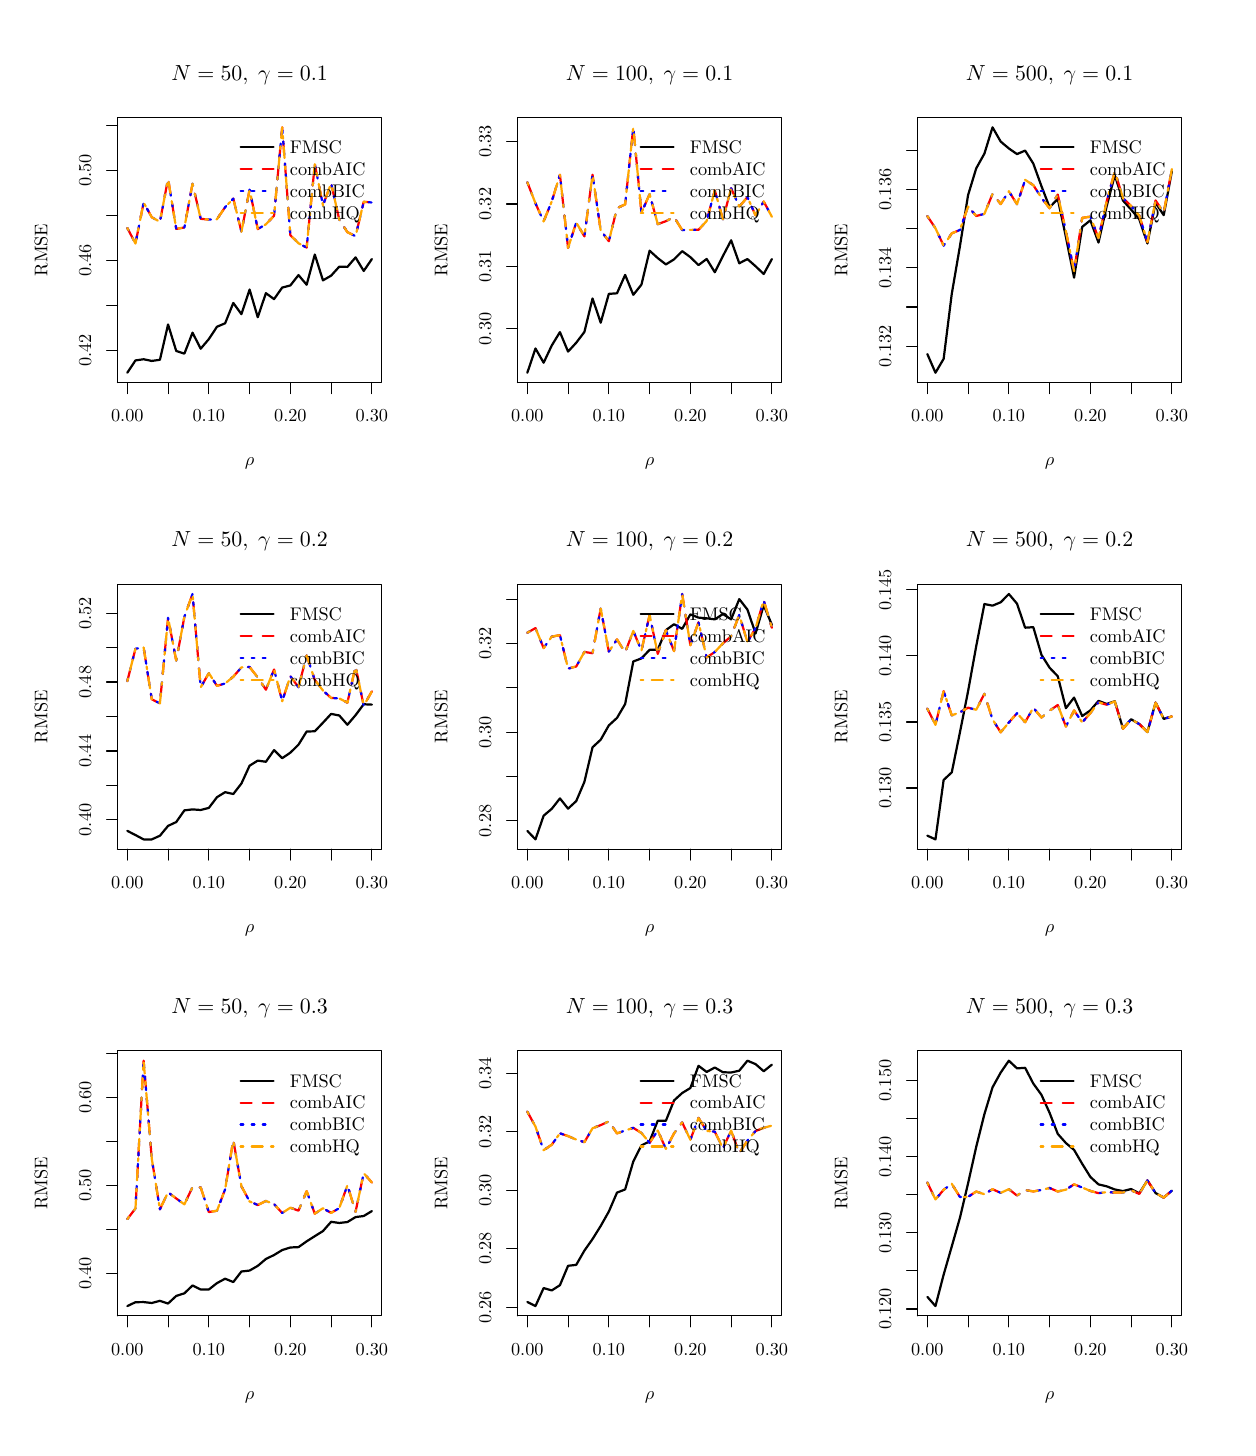
\begin{tikzpicture}[x=1pt,y=1pt]
\definecolor[named]{fillColor}{rgb}{1.00,1.00,1.00}
\path[use as bounding box,fill=fillColor,fill opacity=0.00] (0,0) rectangle (433.62,505.89);
\begin{scope}
\path[clip] ( 32.47,377.65) rectangle (127.91,473.42);
\definecolor[named]{drawColor}{rgb}{0.00,0.00,0.00}

\path[draw=drawColor,line width= 0.8pt,line join=round,line cap=round] ( 36.01,381.20) --
	( 38.95,385.65) --
	( 41.90,386.07) --
	( 44.84,385.46) --
	( 47.79,385.88) --
	( 50.73,398.64) --
	( 53.68,389.07) --
	( 56.63,388.10) --
	( 59.57,395.67) --
	( 62.52,389.88) --
	( 65.46,393.35) --
	( 68.41,397.82) --
	( 71.35,399.07) --
	( 74.30,406.41) --
	( 77.24,402.36) --
	( 80.19,411.27) --
	( 83.14,401.25) --
	( 86.08,409.95) --
	( 89.03,407.80) --
	( 91.97,411.97) --
	( 94.92,412.74) --
	( 97.86,416.48) --
	(100.81,412.99) --
	(103.75,423.90) --
	(106.70,414.58) --
	(109.65,416.27) --
	(112.59,419.53) --
	(115.54,419.44) --
	(118.48,422.88) --
	(121.43,417.97) --
	(124.37,422.27);
\end{scope}
\begin{scope}
\path[clip] (  0.00,  0.00) rectangle (433.62,505.89);
\definecolor[named]{drawColor}{rgb}{0.00,0.00,0.00}

\path[draw=drawColor,line width= 0.4pt,line join=round,line cap=round] ( 36.01,377.65) -- (124.37,377.65);

\path[draw=drawColor,line width= 0.4pt,line join=round,line cap=round] ( 36.01,377.65) -- ( 36.01,373.69);

\path[draw=drawColor,line width= 0.4pt,line join=round,line cap=round] ( 50.73,377.65) -- ( 50.73,373.69);

\path[draw=drawColor,line width= 0.4pt,line join=round,line cap=round] ( 65.46,377.65) -- ( 65.46,373.69);

\path[draw=drawColor,line width= 0.4pt,line join=round,line cap=round] ( 80.19,377.65) -- ( 80.19,373.69);

\path[draw=drawColor,line width= 0.4pt,line join=round,line cap=round] ( 94.92,377.65) -- ( 94.92,373.69);

\path[draw=drawColor,line width= 0.4pt,line join=round,line cap=round] (109.65,377.65) -- (109.65,373.69);

\path[draw=drawColor,line width= 0.4pt,line join=round,line cap=round] (124.37,377.65) -- (124.37,373.69);

\node[text=drawColor,anchor=base,inner sep=0pt, outer sep=0pt, scale=  0.66] at ( 36.01,363.40) {0.00};

\node[text=drawColor,anchor=base,inner sep=0pt, outer sep=0pt, scale=  0.66] at ( 65.46,363.40) {0.10};

\node[text=drawColor,anchor=base,inner sep=0pt, outer sep=0pt, scale=  0.66] at ( 94.92,363.40) {0.20};

\node[text=drawColor,anchor=base,inner sep=0pt, outer sep=0pt, scale=  0.66] at (124.37,363.40) {0.30};

\path[draw=drawColor,line width= 0.4pt,line join=round,line cap=round] ( 32.47,389.34) -- ( 32.47,470.52);

\path[draw=drawColor,line width= 0.4pt,line join=round,line cap=round] ( 32.47,389.34) -- ( 28.51,389.34);

\path[draw=drawColor,line width= 0.4pt,line join=round,line cap=round] ( 32.47,405.58) -- ( 28.51,405.58);

\path[draw=drawColor,line width= 0.4pt,line join=round,line cap=round] ( 32.47,421.82) -- ( 28.51,421.82);

\path[draw=drawColor,line width= 0.4pt,line join=round,line cap=round] ( 32.47,438.05) -- ( 28.51,438.05);

\path[draw=drawColor,line width= 0.4pt,line join=round,line cap=round] ( 32.47,454.29) -- ( 28.51,454.29);

\path[draw=drawColor,line width= 0.4pt,line join=round,line cap=round] ( 32.47,470.52) -- ( 28.51,470.52);

\node[text=drawColor,rotate= 90.00,anchor=base,inner sep=0pt, outer sep=0pt, scale=  0.66] at ( 22.97,389.34) {0.42};

\node[text=drawColor,rotate= 90.00,anchor=base,inner sep=0pt, outer sep=0pt, scale=  0.66] at ( 22.97,421.82) {0.46};

\node[text=drawColor,rotate= 90.00,anchor=base,inner sep=0pt, outer sep=0pt, scale=  0.66] at ( 22.97,454.29) {0.50};

\path[draw=drawColor,line width= 0.4pt,line join=round,line cap=round] ( 32.47,377.65) --
	(127.91,377.65) --
	(127.91,473.42) --
	( 32.47,473.42) --
	( 32.47,377.65);
\end{scope}
\begin{scope}
\path[clip] (  0.00,337.26) rectangle (144.54,505.89);
\definecolor[named]{drawColor}{rgb}{0.00,0.00,0.00}

\node[text=drawColor,anchor=base,inner sep=0pt, outer sep=0pt, scale=  0.79] at ( 80.19,486.92) {\bfseries $N=50, \;\gamma=0.1$};

\node[text=drawColor,anchor=base,inner sep=0pt, outer sep=0pt, scale=  0.66] at ( 80.19,347.56) {$\rho$};

\node[text=drawColor,rotate= 90.00,anchor=base,inner sep=0pt, outer sep=0pt, scale=  0.66] at (  7.13,425.53) {RMSE};
\end{scope}
\begin{scope}
\path[clip] ( 32.47,377.65) rectangle (127.91,473.42);
\definecolor[named]{drawColor}{rgb}{1.00,0.00,0.00}

\path[draw=drawColor,line width= 0.8pt,dash pattern=on 4pt off 4pt ,line join=round,line cap=round] ( 36.01,433.50) --
	( 38.95,427.87) --
	( 41.90,442.68) --
	( 44.84,437.38) --
	( 47.79,435.74) --
	( 50.73,451.33) --
	( 53.68,433.17) --
	( 56.63,433.68) --
	( 59.57,449.52) --
	( 62.52,436.82) --
	( 65.46,436.53) --
	( 68.41,436.69) --
	( 71.35,441.03) --
	( 74.30,444.11) --
	( 77.24,432.14) --
	( 80.19,447.38) --
	( 83.14,433.11) --
	( 86.08,434.83) --
	( 89.03,437.92) --
	( 91.97,469.87) --
	( 94.92,430.89) --
	( 97.86,427.98) --
	(100.81,426.42) --
	(103.75,456.54) --
	(106.70,441.70) --
	(109.65,449.62) --
	(112.59,436.54) --
	(115.54,431.98) --
	(118.48,430.54) --
	(121.43,442.97) --
	(124.37,442.71);
\definecolor[named]{drawColor}{rgb}{0.00,0.00,1.00}

\path[draw=drawColor,line width= 0.8pt,dash pattern=on 1pt off 3pt ,line join=round,line cap=round] ( 36.01,433.50) --
	( 38.95,427.87) --
	( 41.90,442.68) --
	( 44.84,437.38) --
	( 47.79,435.74) --
	( 50.73,451.33) --
	( 53.68,433.17) --
	( 56.63,433.68) --
	( 59.57,449.52) --
	( 62.52,436.82) --
	( 65.46,436.53) --
	( 68.41,436.69) --
	( 71.35,441.03) --
	( 74.30,444.11) --
	( 77.24,432.14) --
	( 80.19,447.38) --
	( 83.14,433.11) --
	( 86.08,434.83) --
	( 89.03,437.92) --
	( 91.97,469.87) --
	( 94.92,430.89) --
	( 97.86,427.98) --
	(100.81,426.42) --
	(103.75,456.54) --
	(106.70,441.70) --
	(109.65,449.62) --
	(112.59,436.54) --
	(115.54,431.98) --
	(118.48,430.54) --
	(121.43,442.97) --
	(124.37,442.71);
\definecolor[named]{drawColor}{rgb}{1.00,0.65,0.00}

\path[draw=drawColor,line width= 0.8pt,dash pattern=on 1pt off 3pt on 4pt off 3pt ,line join=round,line cap=round] ( 36.01,433.50) --
	( 38.95,427.87) --
	( 41.90,442.68) --
	( 44.84,437.38) --
	( 47.79,435.74) --
	( 50.73,451.33) --
	( 53.68,433.17) --
	( 56.63,433.68) --
	( 59.57,449.52) --
	( 62.52,436.82) --
	( 65.46,436.53) --
	( 68.41,436.69) --
	( 71.35,441.03) --
	( 74.30,444.11) --
	( 77.24,432.14) --
	( 80.19,447.38) --
	( 83.14,433.11) --
	( 86.08,434.83) --
	( 89.03,437.92) --
	( 91.97,469.87) --
	( 94.92,430.89) --
	( 97.86,427.98) --
	(100.81,426.42) --
	(103.75,456.54) --
	(106.70,441.70) --
	(109.65,449.62) --
	(112.59,436.54) --
	(115.54,431.98) --
	(118.48,430.54) --
	(121.43,442.97) --
	(124.37,442.71);
\definecolor[named]{drawColor}{rgb}{0.00,0.00,0.00}

\path[draw=drawColor,line width= 0.8pt,line join=round,line cap=round] ( 76.94,462.63) -- ( 88.82,462.63);
\definecolor[named]{drawColor}{rgb}{1.00,0.00,0.00}

\path[draw=drawColor,line width= 0.8pt,dash pattern=on 4pt off 4pt ,line join=round,line cap=round] ( 76.94,454.71) -- ( 88.82,454.71);
\definecolor[named]{drawColor}{rgb}{0.00,0.00,1.00}

\path[draw=drawColor,line width= 0.8pt,dash pattern=on 1pt off 3pt ,line join=round,line cap=round] ( 76.94,446.79) -- ( 88.82,446.79);
\definecolor[named]{drawColor}{rgb}{1.00,0.65,0.00}

\path[draw=drawColor,line width= 0.8pt,dash pattern=on 1pt off 3pt on 4pt off 3pt ,line join=round,line cap=round] ( 76.94,438.87) -- ( 88.82,438.87);
\definecolor[named]{drawColor}{rgb}{0.00,0.00,0.00}

\node[text=drawColor,anchor=base west,inner sep=0pt, outer sep=0pt, scale=  0.66] at ( 94.76,460.35) {FMSC};

\node[text=drawColor,anchor=base west,inner sep=0pt, outer sep=0pt, scale=  0.66] at ( 94.76,452.43) {combAIC};

\node[text=drawColor,anchor=base west,inner sep=0pt, outer sep=0pt, scale=  0.66] at ( 94.76,444.51) {combBIC};

\node[text=drawColor,anchor=base west,inner sep=0pt, outer sep=0pt, scale=  0.66] at ( 94.76,436.59) {combHQ};
\end{scope}
\begin{scope}
\path[clip] (177.01,377.65) rectangle (272.45,473.42);
\definecolor[named]{drawColor}{rgb}{0.00,0.00,0.00}

\path[draw=drawColor,line width= 0.8pt,line join=round,line cap=round] (180.55,381.20) --
	(183.49,389.97) --
	(186.44,384.82) --
	(189.38,391.05) --
	(192.33,395.88) --
	(195.27,388.83) --
	(198.22,392.05) --
	(201.17,395.92) --
	(204.11,408.04) --
	(207.06,399.28) --
	(210.00,409.69) --
	(212.95,409.90) --
	(215.89,416.55) --
	(218.84,409.36) --
	(221.78,413.03) --
	(224.73,425.30) --
	(227.68,422.62) --
	(230.62,420.34) --
	(233.57,422.16) --
	(236.51,425.14) --
	(239.46,422.96) --
	(242.40,420.10) --
	(245.35,422.31) --
	(248.29,417.51) --
	(251.24,423.40) --
	(254.19,429.05) --
	(257.13,420.75) --
	(260.08,422.27) --
	(263.02,419.68) --
	(265.97,416.87) --
	(268.91,422.27);
\end{scope}
\begin{scope}
\path[clip] (  0.00,  0.00) rectangle (433.62,505.89);
\definecolor[named]{drawColor}{rgb}{0.00,0.00,0.00}

\path[draw=drawColor,line width= 0.4pt,line join=round,line cap=round] (180.55,377.65) -- (268.91,377.65);

\path[draw=drawColor,line width= 0.4pt,line join=round,line cap=round] (180.55,377.65) -- (180.55,373.69);

\path[draw=drawColor,line width= 0.4pt,line join=round,line cap=round] (195.27,377.65) -- (195.27,373.69);

\path[draw=drawColor,line width= 0.4pt,line join=round,line cap=round] (210.00,377.65) -- (210.00,373.69);

\path[draw=drawColor,line width= 0.4pt,line join=round,line cap=round] (224.73,377.65) -- (224.73,373.69);

\path[draw=drawColor,line width= 0.4pt,line join=round,line cap=round] (239.46,377.65) -- (239.46,373.69);

\path[draw=drawColor,line width= 0.4pt,line join=round,line cap=round] (254.19,377.65) -- (254.19,373.69);

\path[draw=drawColor,line width= 0.4pt,line join=round,line cap=round] (268.91,377.65) -- (268.91,373.69);

\node[text=drawColor,anchor=base,inner sep=0pt, outer sep=0pt, scale=  0.66] at (180.55,363.40) {0.00};

\node[text=drawColor,anchor=base,inner sep=0pt, outer sep=0pt, scale=  0.66] at (210.00,363.40) {0.10};

\node[text=drawColor,anchor=base,inner sep=0pt, outer sep=0pt, scale=  0.66] at (239.46,363.40) {0.20};

\node[text=drawColor,anchor=base,inner sep=0pt, outer sep=0pt, scale=  0.66] at (268.91,363.40) {0.30};

\path[draw=drawColor,line width= 0.4pt,line join=round,line cap=round] (177.01,397.02) -- (177.01,464.76);

\path[draw=drawColor,line width= 0.4pt,line join=round,line cap=round] (177.01,397.02) -- (173.05,397.02);

\path[draw=drawColor,line width= 0.4pt,line join=round,line cap=round] (177.01,419.60) -- (173.05,419.60);

\path[draw=drawColor,line width= 0.4pt,line join=round,line cap=round] (177.01,442.18) -- (173.05,442.18);

\path[draw=drawColor,line width= 0.4pt,line join=round,line cap=round] (177.01,464.76) -- (173.05,464.76);

\node[text=drawColor,rotate= 90.00,anchor=base,inner sep=0pt, outer sep=0pt, scale=  0.66] at (167.51,397.02) {0.30};

\node[text=drawColor,rotate= 90.00,anchor=base,inner sep=0pt, outer sep=0pt, scale=  0.66] at (167.51,419.60) {0.31};

\node[text=drawColor,rotate= 90.00,anchor=base,inner sep=0pt, outer sep=0pt, scale=  0.66] at (167.51,442.18) {0.32};

\node[text=drawColor,rotate= 90.00,anchor=base,inner sep=0pt, outer sep=0pt, scale=  0.66] at (167.51,464.76) {0.33};

\path[draw=drawColor,line width= 0.4pt,line join=round,line cap=round] (177.01,377.65) --
	(272.45,377.65) --
	(272.45,473.42) --
	(177.01,473.42) --
	(177.01,377.65);
\end{scope}
\begin{scope}
\path[clip] (144.54,337.26) rectangle (289.08,505.89);
\definecolor[named]{drawColor}{rgb}{0.00,0.00,0.00}

\node[text=drawColor,anchor=base,inner sep=0pt, outer sep=0pt, scale=  0.79] at (224.73,486.92) {\bfseries $N=100, \;\gamma=0.1$};

\node[text=drawColor,anchor=base,inner sep=0pt, outer sep=0pt, scale=  0.66] at (224.73,347.56) {$\rho$};

\node[text=drawColor,rotate= 90.00,anchor=base,inner sep=0pt, outer sep=0pt, scale=  0.66] at (151.67,425.53) {RMSE};
\end{scope}
\begin{scope}
\path[clip] (177.01,377.65) rectangle (272.45,473.42);
\definecolor[named]{drawColor}{rgb}{1.00,0.00,0.00}

\path[draw=drawColor,line width= 0.8pt,dash pattern=on 4pt off 4pt ,line join=round,line cap=round] (180.55,450.01) --
	(183.49,442.42) --
	(186.44,435.86) --
	(189.38,443.13) --
	(192.33,452.74) --
	(195.27,426.31) --
	(198.22,435.48) --
	(201.17,430.46) --
	(204.11,452.76) --
	(207.06,432.61) --
	(210.00,428.73) --
	(212.95,440.66) --
	(215.89,442.03) --
	(218.84,469.87) --
	(221.78,438.98) --
	(224.73,445.76) --
	(227.68,434.89) --
	(230.62,435.96) --
	(233.57,437.46) --
	(236.51,432.72) --
	(239.46,432.82) --
	(242.40,432.83) --
	(245.35,436.03) --
	(248.29,447.08) --
	(251.24,436.61) --
	(254.19,447.86) --
	(257.13,441.21) --
	(260.08,444.64) --
	(263.02,438.06) --
	(265.97,443.06) --
	(268.91,437.55);
\definecolor[named]{drawColor}{rgb}{0.00,0.00,1.00}

\path[draw=drawColor,line width= 0.8pt,dash pattern=on 1pt off 3pt ,line join=round,line cap=round] (180.55,450.01) --
	(183.49,442.42) --
	(186.44,435.86) --
	(189.38,443.13) --
	(192.33,452.74) --
	(195.27,426.31) --
	(198.22,435.48) --
	(201.17,430.46) --
	(204.11,452.76) --
	(207.06,432.61) --
	(210.00,428.73) --
	(212.95,440.66) --
	(215.89,442.03) --
	(218.84,469.87) --
	(221.78,438.98) --
	(224.73,445.76) --
	(227.68,434.89) --
	(230.62,435.96) --
	(233.57,437.46) --
	(236.51,432.72) --
	(239.46,432.82) --
	(242.40,432.83) --
	(245.35,436.03) --
	(248.29,447.08) --
	(251.24,436.61) --
	(254.19,447.86) --
	(257.13,441.21) --
	(260.08,444.64) --
	(263.02,438.06) --
	(265.97,443.06) --
	(268.91,437.55);
\definecolor[named]{drawColor}{rgb}{1.00,0.65,0.00}

\path[draw=drawColor,line width= 0.8pt,dash pattern=on 1pt off 3pt on 4pt off 3pt ,line join=round,line cap=round] (180.55,450.01) --
	(183.49,442.42) --
	(186.44,435.86) --
	(189.38,443.13) --
	(192.33,452.74) --
	(195.27,426.31) --
	(198.22,435.48) --
	(201.17,430.46) --
	(204.11,452.76) --
	(207.06,432.61) --
	(210.00,428.73) --
	(212.95,440.66) --
	(215.89,442.03) --
	(218.84,469.87) --
	(221.78,438.98) --
	(224.73,445.76) --
	(227.68,434.89) --
	(230.62,435.96) --
	(233.57,437.46) --
	(236.51,432.72) --
	(239.46,432.82) --
	(242.40,432.83) --
	(245.35,436.03) --
	(248.29,447.08) --
	(251.24,436.61) --
	(254.19,447.86) --
	(257.13,441.21) --
	(260.08,444.64) --
	(263.02,438.06) --
	(265.97,443.06) --
	(268.91,437.55);
\definecolor[named]{drawColor}{rgb}{0.00,0.00,0.00}

\path[draw=drawColor,line width= 0.8pt,line join=round,line cap=round] (221.48,462.63) -- (233.36,462.63);
\definecolor[named]{drawColor}{rgb}{1.00,0.00,0.00}

\path[draw=drawColor,line width= 0.8pt,dash pattern=on 4pt off 4pt ,line join=round,line cap=round] (221.48,454.71) -- (233.36,454.71);
\definecolor[named]{drawColor}{rgb}{0.00,0.00,1.00}

\path[draw=drawColor,line width= 0.8pt,dash pattern=on 1pt off 3pt ,line join=round,line cap=round] (221.48,446.79) -- (233.36,446.79);
\definecolor[named]{drawColor}{rgb}{1.00,0.65,0.00}

\path[draw=drawColor,line width= 0.8pt,dash pattern=on 1pt off 3pt on 4pt off 3pt ,line join=round,line cap=round] (221.48,438.87) -- (233.36,438.87);
\definecolor[named]{drawColor}{rgb}{0.00,0.00,0.00}

\node[text=drawColor,anchor=base west,inner sep=0pt, outer sep=0pt, scale=  0.66] at (239.30,460.35) {FMSC};

\node[text=drawColor,anchor=base west,inner sep=0pt, outer sep=0pt, scale=  0.66] at (239.30,452.43) {combAIC};

\node[text=drawColor,anchor=base west,inner sep=0pt, outer sep=0pt, scale=  0.66] at (239.30,444.51) {combBIC};

\node[text=drawColor,anchor=base west,inner sep=0pt, outer sep=0pt, scale=  0.66] at (239.30,436.59) {combHQ};
\end{scope}
\begin{scope}
\path[clip] (321.55,377.65) rectangle (416.99,473.42);
\definecolor[named]{drawColor}{rgb}{0.00,0.00,0.00}

\path[draw=drawColor,line width= 0.8pt,line join=round,line cap=round] (325.09,387.95) --
	(328.03,381.20) --
	(330.98,386.22) --
	(333.92,409.71) --
	(336.87,426.93) --
	(339.81,445.39) --
	(342.76,455.07) --
	(345.71,460.37) --
	(348.65,469.87) --
	(351.60,464.72) --
	(354.54,462.25) --
	(357.49,460.20) --
	(360.43,461.47) --
	(363.38,456.77) --
	(366.32,448.63) --
	(369.27,440.98) --
	(372.22,444.00) --
	(375.16,430.27) --
	(378.11,415.55) --
	(381.05,433.89) --
	(384.00,436.29) --
	(386.94,428.24) --
	(389.89,441.36) --
	(392.83,452.57) --
	(395.78,443.41) --
	(398.73,440.14) --
	(401.67,436.66) --
	(404.62,427.91) --
	(407.56,442.63) --
	(410.51,438.12) --
	(413.45,454.01);
\end{scope}
\begin{scope}
\path[clip] (  0.00,  0.00) rectangle (433.62,505.89);
\definecolor[named]{drawColor}{rgb}{0.00,0.00,0.00}

\path[draw=drawColor,line width= 0.4pt,line join=round,line cap=round] (325.09,377.65) -- (413.45,377.65);

\path[draw=drawColor,line width= 0.4pt,line join=round,line cap=round] (325.09,377.65) -- (325.09,373.69);

\path[draw=drawColor,line width= 0.4pt,line join=round,line cap=round] (339.81,377.65) -- (339.81,373.69);

\path[draw=drawColor,line width= 0.4pt,line join=round,line cap=round] (354.54,377.65) -- (354.54,373.69);

\path[draw=drawColor,line width= 0.4pt,line join=round,line cap=round] (369.27,377.65) -- (369.27,373.69);

\path[draw=drawColor,line width= 0.4pt,line join=round,line cap=round] (384.00,377.65) -- (384.00,373.69);

\path[draw=drawColor,line width= 0.4pt,line join=round,line cap=round] (398.73,377.65) -- (398.73,373.69);

\path[draw=drawColor,line width= 0.4pt,line join=round,line cap=round] (413.45,377.65) -- (413.45,373.69);

\node[text=drawColor,anchor=base,inner sep=0pt, outer sep=0pt, scale=  0.66] at (325.09,363.40) {0.00};

\node[text=drawColor,anchor=base,inner sep=0pt, outer sep=0pt, scale=  0.66] at (354.54,363.40) {0.10};

\node[text=drawColor,anchor=base,inner sep=0pt, outer sep=0pt, scale=  0.66] at (384.00,363.40) {0.20};

\node[text=drawColor,anchor=base,inner sep=0pt, outer sep=0pt, scale=  0.66] at (413.45,363.40) {0.30};

\path[draw=drawColor,line width= 0.4pt,line join=round,line cap=round] (321.55,390.79) -- (321.55,461.58);

\path[draw=drawColor,line width= 0.4pt,line join=round,line cap=round] (321.55,390.79) -- (317.59,390.79);

\path[draw=drawColor,line width= 0.4pt,line join=round,line cap=round] (321.55,404.94) -- (317.59,404.94);

\path[draw=drawColor,line width= 0.4pt,line join=round,line cap=round] (321.55,419.10) -- (317.59,419.10);

\path[draw=drawColor,line width= 0.4pt,line join=round,line cap=round] (321.55,433.26) -- (317.59,433.26);

\path[draw=drawColor,line width= 0.4pt,line join=round,line cap=round] (321.55,447.42) -- (317.59,447.42);

\path[draw=drawColor,line width= 0.4pt,line join=round,line cap=round] (321.55,461.58) -- (317.59,461.58);

\node[text=drawColor,rotate= 90.00,anchor=base,inner sep=0pt, outer sep=0pt, scale=  0.66] at (312.05,390.79) {0.132};

\node[text=drawColor,rotate= 90.00,anchor=base,inner sep=0pt, outer sep=0pt, scale=  0.66] at (312.05,419.10) {0.134};

\node[text=drawColor,rotate= 90.00,anchor=base,inner sep=0pt, outer sep=0pt, scale=  0.66] at (312.05,447.42) {0.136};

\path[draw=drawColor,line width= 0.4pt,line join=round,line cap=round] (321.55,377.65) --
	(416.99,377.65) --
	(416.99,473.42) --
	(321.55,473.42) --
	(321.55,377.65);
\end{scope}
\begin{scope}
\path[clip] (289.08,337.26) rectangle (433.62,505.89);
\definecolor[named]{drawColor}{rgb}{0.00,0.00,0.00}

\node[text=drawColor,anchor=base,inner sep=0pt, outer sep=0pt, scale=  0.79] at (369.27,486.92) {\bfseries $N=500, \;\gamma=0.1$};

\node[text=drawColor,anchor=base,inner sep=0pt, outer sep=0pt, scale=  0.66] at (369.27,347.56) {$\rho$};

\node[text=drawColor,rotate= 90.00,anchor=base,inner sep=0pt, outer sep=0pt, scale=  0.66] at (296.21,425.53) {RMSE};
\end{scope}
\begin{scope}
\path[clip] (321.55,377.65) rectangle (416.99,473.42);
\definecolor[named]{drawColor}{rgb}{1.00,0.00,0.00}

\path[draw=drawColor,line width= 0.8pt,dash pattern=on 4pt off 4pt ,line join=round,line cap=round] (325.09,437.79) --
	(328.03,433.38) --
	(330.98,427.10) --
	(333.92,431.57) --
	(336.87,432.79) --
	(339.81,441.24) --
	(342.76,437.84) --
	(345.71,438.60) --
	(348.65,445.81) --
	(351.60,442.14) --
	(354.54,446.78) --
	(357.49,442.09) --
	(360.43,450.89) --
	(363.38,448.99) --
	(366.32,444.42) --
	(369.27,440.61) --
	(372.22,445.58) --
	(375.16,432.35) --
	(378.11,417.93) --
	(381.05,437.16) --
	(384.00,437.60) --
	(386.94,429.78) --
	(389.89,443.11) --
	(392.83,453.95) --
	(395.78,444.31) --
	(398.73,441.40) --
	(401.67,438.01) --
	(404.62,428.42) --
	(407.56,443.45) --
	(410.51,439.04) --
	(413.45,454.79);
\definecolor[named]{drawColor}{rgb}{0.00,0.00,1.00}

\path[draw=drawColor,line width= 0.8pt,dash pattern=on 1pt off 3pt ,line join=round,line cap=round] (325.09,437.79) --
	(328.03,433.38) --
	(330.98,427.10) --
	(333.92,431.57) --
	(336.87,432.79) --
	(339.81,441.24) --
	(342.76,437.84) --
	(345.71,438.60) --
	(348.65,445.81) --
	(351.60,442.14) --
	(354.54,446.78) --
	(357.49,442.09) --
	(360.43,450.89) --
	(363.38,448.99) --
	(366.32,444.42) --
	(369.27,440.61) --
	(372.22,445.58) --
	(375.16,432.35) --
	(378.11,417.93) --
	(381.05,437.16) --
	(384.00,437.60) --
	(386.94,429.78) --
	(389.89,443.11) --
	(392.83,453.95) --
	(395.78,444.31) --
	(398.73,441.40) --
	(401.67,438.01) --
	(404.62,428.42) --
	(407.56,443.45) --
	(410.51,439.04) --
	(413.45,454.79);
\definecolor[named]{drawColor}{rgb}{1.00,0.65,0.00}

\path[draw=drawColor,line width= 0.8pt,dash pattern=on 1pt off 3pt on 4pt off 3pt ,line join=round,line cap=round] (325.09,437.79) --
	(328.03,433.38) --
	(330.98,427.10) --
	(333.92,431.57) --
	(336.87,432.79) --
	(339.81,441.24) --
	(342.76,437.84) --
	(345.71,438.60) --
	(348.65,445.81) --
	(351.60,442.14) --
	(354.54,446.78) --
	(357.49,442.09) --
	(360.43,450.89) --
	(363.38,448.99) --
	(366.32,444.42) --
	(369.27,440.61) --
	(372.22,445.58) --
	(375.16,432.35) --
	(378.11,417.93) --
	(381.05,437.16) --
	(384.00,437.60) --
	(386.94,429.78) --
	(389.89,443.11) --
	(392.83,453.95) --
	(395.78,444.31) --
	(398.73,441.40) --
	(401.67,438.01) --
	(404.62,428.42) --
	(407.56,443.45) --
	(410.51,439.04) --
	(413.45,454.79);
\definecolor[named]{drawColor}{rgb}{0.00,0.00,0.00}

\path[draw=drawColor,line width= 0.8pt,line join=round,line cap=round] (366.02,462.63) -- (377.90,462.63);
\definecolor[named]{drawColor}{rgb}{1.00,0.00,0.00}

\path[draw=drawColor,line width= 0.8pt,dash pattern=on 4pt off 4pt ,line join=round,line cap=round] (366.02,454.71) -- (377.90,454.71);
\definecolor[named]{drawColor}{rgb}{0.00,0.00,1.00}

\path[draw=drawColor,line width= 0.8pt,dash pattern=on 1pt off 3pt ,line join=round,line cap=round] (366.02,446.79) -- (377.90,446.79);
\definecolor[named]{drawColor}{rgb}{1.00,0.65,0.00}

\path[draw=drawColor,line width= 0.8pt,dash pattern=on 1pt off 3pt on 4pt off 3pt ,line join=round,line cap=round] (366.02,438.87) -- (377.90,438.87);
\definecolor[named]{drawColor}{rgb}{0.00,0.00,0.00}

\node[text=drawColor,anchor=base west,inner sep=0pt, outer sep=0pt, scale=  0.66] at (383.84,460.35) {FMSC};

\node[text=drawColor,anchor=base west,inner sep=0pt, outer sep=0pt, scale=  0.66] at (383.84,452.43) {combAIC};

\node[text=drawColor,anchor=base west,inner sep=0pt, outer sep=0pt, scale=  0.66] at (383.84,444.51) {combBIC};

\node[text=drawColor,anchor=base west,inner sep=0pt, outer sep=0pt, scale=  0.66] at (383.84,436.59) {combHQ};
\end{scope}
\begin{scope}
\path[clip] ( 32.47,209.02) rectangle (127.91,304.79);
\definecolor[named]{drawColor}{rgb}{0.00,0.00,0.00}

\path[draw=drawColor,line width= 0.8pt,line join=round,line cap=round] ( 36.01,215.65) --
	( 38.95,214.14) --
	( 41.90,212.57) --
	( 44.84,212.57) --
	( 47.79,213.90) --
	( 50.73,217.45) --
	( 53.68,218.84) --
	( 56.63,223.06) --
	( 59.57,223.41) --
	( 62.52,223.20) --
	( 65.46,223.95) --
	( 68.41,227.83) --
	( 71.35,229.63) --
	( 74.30,228.97) --
	( 77.24,232.77) --
	( 80.19,239.21) --
	( 83.14,241.04) --
	( 86.08,240.62) --
	( 89.03,244.84) --
	( 91.97,241.92) --
	( 94.92,243.91) --
	( 97.86,246.80) --
	(100.81,251.56) --
	(103.75,251.63) --
	(106.70,254.73) --
	(109.65,257.92) --
	(112.59,257.35) --
	(115.54,253.99) --
	(118.48,257.46) --
	(121.43,261.40) --
	(124.37,261.27);
\end{scope}
\begin{scope}
\path[clip] (  0.00,  0.00) rectangle (433.62,505.89);
\definecolor[named]{drawColor}{rgb}{0.00,0.00,0.00}

\path[draw=drawColor,line width= 0.4pt,line join=round,line cap=round] ( 36.01,209.02) -- (124.37,209.02);

\path[draw=drawColor,line width= 0.4pt,line join=round,line cap=round] ( 36.01,209.02) -- ( 36.01,205.06);

\path[draw=drawColor,line width= 0.4pt,line join=round,line cap=round] ( 50.73,209.02) -- ( 50.73,205.06);

\path[draw=drawColor,line width= 0.4pt,line join=round,line cap=round] ( 65.46,209.02) -- ( 65.46,205.06);

\path[draw=drawColor,line width= 0.4pt,line join=round,line cap=round] ( 80.19,209.02) -- ( 80.19,205.06);

\path[draw=drawColor,line width= 0.4pt,line join=round,line cap=round] ( 94.92,209.02) -- ( 94.92,205.06);

\path[draw=drawColor,line width= 0.4pt,line join=round,line cap=round] (109.65,209.02) -- (109.65,205.06);

\path[draw=drawColor,line width= 0.4pt,line join=round,line cap=round] (124.37,209.02) -- (124.37,205.06);

\node[text=drawColor,anchor=base,inner sep=0pt, outer sep=0pt, scale=  0.66] at ( 36.01,194.77) {0.00};

\node[text=drawColor,anchor=base,inner sep=0pt, outer sep=0pt, scale=  0.66] at ( 65.46,194.77) {0.10};

\node[text=drawColor,anchor=base,inner sep=0pt, outer sep=0pt, scale=  0.66] at ( 94.92,194.77) {0.20};

\node[text=drawColor,anchor=base,inner sep=0pt, outer sep=0pt, scale=  0.66] at (124.37,194.77) {0.30};

\path[draw=drawColor,line width= 0.4pt,line join=round,line cap=round] ( 32.47,219.62) -- ( 32.47,294.33);

\path[draw=drawColor,line width= 0.4pt,line join=round,line cap=round] ( 32.47,219.62) -- ( 28.51,219.62);

\path[draw=drawColor,line width= 0.4pt,line join=round,line cap=round] ( 32.47,232.07) -- ( 28.51,232.07);

\path[draw=drawColor,line width= 0.4pt,line join=round,line cap=round] ( 32.47,244.52) -- ( 28.51,244.52);

\path[draw=drawColor,line width= 0.4pt,line join=round,line cap=round] ( 32.47,256.97) -- ( 28.51,256.97);

\path[draw=drawColor,line width= 0.4pt,line join=round,line cap=round] ( 32.47,269.43) -- ( 28.51,269.43);

\path[draw=drawColor,line width= 0.4pt,line join=round,line cap=round] ( 32.47,281.88) -- ( 28.51,281.88);

\path[draw=drawColor,line width= 0.4pt,line join=round,line cap=round] ( 32.47,294.33) -- ( 28.51,294.33);

\node[text=drawColor,rotate= 90.00,anchor=base,inner sep=0pt, outer sep=0pt, scale=  0.66] at ( 22.97,219.62) {0.40};

\node[text=drawColor,rotate= 90.00,anchor=base,inner sep=0pt, outer sep=0pt, scale=  0.66] at ( 22.97,244.52) {0.44};

\node[text=drawColor,rotate= 90.00,anchor=base,inner sep=0pt, outer sep=0pt, scale=  0.66] at ( 22.97,269.43) {0.48};

\node[text=drawColor,rotate= 90.00,anchor=base,inner sep=0pt, outer sep=0pt, scale=  0.66] at ( 22.97,294.33) {0.52};

\path[draw=drawColor,line width= 0.4pt,line join=round,line cap=round] ( 32.47,209.02) --
	(127.91,209.02) --
	(127.91,304.79) --
	( 32.47,304.79) --
	( 32.47,209.02);
\end{scope}
\begin{scope}
\path[clip] (  0.00,168.63) rectangle (144.54,337.26);
\definecolor[named]{drawColor}{rgb}{0.00,0.00,0.00}

\node[text=drawColor,anchor=base,inner sep=0pt, outer sep=0pt, scale=  0.79] at ( 80.19,318.29) {\bfseries $N=50, \;\gamma=0.2$};

\node[text=drawColor,anchor=base,inner sep=0pt, outer sep=0pt, scale=  0.66] at ( 80.19,178.93) {$\rho$};

\node[text=drawColor,rotate= 90.00,anchor=base,inner sep=0pt, outer sep=0pt, scale=  0.66] at (  7.13,256.90) {RMSE};
\end{scope}
\begin{scope}
\path[clip] ( 32.47,209.02) rectangle (127.91,304.79);
\definecolor[named]{drawColor}{rgb}{1.00,0.00,0.00}

\path[draw=drawColor,line width= 0.8pt,dash pattern=on 4pt off 4pt ,line join=round,line cap=round] ( 36.01,269.76) --
	( 38.95,281.47) --
	( 41.90,281.92) --
	( 44.84,263.21) --
	( 47.79,261.71) --
	( 50.73,292.64) --
	( 53.68,277.16) --
	( 56.63,293.04) --
	( 59.57,301.24) --
	( 62.52,267.50) --
	( 65.46,272.65) --
	( 68.41,268.05) --
	( 71.35,268.92) --
	( 74.30,271.36) --
	( 77.24,274.73) --
	( 80.19,274.85) --
	( 83.14,271.09) --
	( 86.08,266.66) --
	( 89.03,273.95) --
	( 91.97,262.49) --
	( 94.92,271.54) --
	( 97.86,267.54) --
	(100.81,279.05) --
	(103.75,270.19) --
	(106.70,266.38) --
	(109.65,263.68) --
	(112.59,263.51) --
	(115.54,261.99) --
	(118.48,275.14) --
	(121.43,260.85) --
	(124.37,266.06);
\definecolor[named]{drawColor}{rgb}{0.00,0.00,1.00}

\path[draw=drawColor,line width= 0.8pt,dash pattern=on 1pt off 3pt ,line join=round,line cap=round] ( 36.01,269.76) --
	( 38.95,281.47) --
	( 41.90,281.92) --
	( 44.84,263.21) --
	( 47.79,261.71) --
	( 50.73,292.64) --
	( 53.68,277.16) --
	( 56.63,293.04) --
	( 59.57,301.24) --
	( 62.52,267.50) --
	( 65.46,272.65) --
	( 68.41,268.05) --
	( 71.35,268.92) --
	( 74.30,271.36) --
	( 77.24,274.73) --
	( 80.19,274.85) --
	( 83.14,271.09) --
	( 86.08,266.66) --
	( 89.03,273.95) --
	( 91.97,262.49) --
	( 94.92,271.54) --
	( 97.86,267.54) --
	(100.81,279.05) --
	(103.75,270.19) --
	(106.70,266.38) --
	(109.65,263.68) --
	(112.59,263.51) --
	(115.54,261.99) --
	(118.48,275.14) --
	(121.43,260.85) --
	(124.37,266.06);
\definecolor[named]{drawColor}{rgb}{1.00,0.65,0.00}

\path[draw=drawColor,line width= 0.8pt,dash pattern=on 1pt off 3pt on 4pt off 3pt ,line join=round,line cap=round] ( 36.01,269.76) --
	( 38.95,281.47) --
	( 41.90,281.92) --
	( 44.84,263.21) --
	( 47.79,261.71) --
	( 50.73,292.64) --
	( 53.68,277.16) --
	( 56.63,293.04) --
	( 59.57,301.24) --
	( 62.52,267.50) --
	( 65.46,272.65) --
	( 68.41,268.05) --
	( 71.35,268.92) --
	( 74.30,271.36) --
	( 77.24,274.73) --
	( 80.19,274.85) --
	( 83.14,271.09) --
	( 86.08,266.66) --
	( 89.03,273.95) --
	( 91.97,262.49) --
	( 94.92,271.54) --
	( 97.86,267.54) --
	(100.81,279.05) --
	(103.75,270.19) --
	(106.70,266.38) --
	(109.65,263.68) --
	(112.59,263.51) --
	(115.54,261.99) --
	(118.48,275.14) --
	(121.43,260.85) --
	(124.37,266.06);
\definecolor[named]{drawColor}{rgb}{0.00,0.00,0.00}

\path[draw=drawColor,line width= 0.8pt,line join=round,line cap=round] ( 76.94,294.00) -- ( 88.82,294.00);
\definecolor[named]{drawColor}{rgb}{1.00,0.00,0.00}

\path[draw=drawColor,line width= 0.8pt,dash pattern=on 4pt off 4pt ,line join=round,line cap=round] ( 76.94,286.08) -- ( 88.82,286.08);
\definecolor[named]{drawColor}{rgb}{0.00,0.00,1.00}

\path[draw=drawColor,line width= 0.8pt,dash pattern=on 1pt off 3pt ,line join=round,line cap=round] ( 76.94,278.16) -- ( 88.82,278.16);
\definecolor[named]{drawColor}{rgb}{1.00,0.65,0.00}

\path[draw=drawColor,line width= 0.8pt,dash pattern=on 1pt off 3pt on 4pt off 3pt ,line join=round,line cap=round] ( 76.94,270.24) -- ( 88.82,270.24);
\definecolor[named]{drawColor}{rgb}{0.00,0.00,0.00}

\node[text=drawColor,anchor=base west,inner sep=0pt, outer sep=0pt, scale=  0.66] at ( 94.76,291.72) {FMSC};

\node[text=drawColor,anchor=base west,inner sep=0pt, outer sep=0pt, scale=  0.66] at ( 94.76,283.80) {combAIC};

\node[text=drawColor,anchor=base west,inner sep=0pt, outer sep=0pt, scale=  0.66] at ( 94.76,275.88) {combBIC};

\node[text=drawColor,anchor=base west,inner sep=0pt, outer sep=0pt, scale=  0.66] at ( 94.76,267.96) {combHQ};
\end{scope}
\begin{scope}
\path[clip] (177.01,209.02) rectangle (272.45,304.79);
\definecolor[named]{drawColor}{rgb}{0.00,0.00,0.00}

\path[draw=drawColor,line width= 0.8pt,line join=round,line cap=round] (180.55,215.65) --
	(183.49,212.57) --
	(186.44,221.14) --
	(189.38,223.62) --
	(192.33,227.38) --
	(195.27,223.68) --
	(198.22,226.42) --
	(201.17,233.36) --
	(204.11,245.85) --
	(207.06,248.59) --
	(210.00,253.76) --
	(212.95,256.47) --
	(215.89,261.47) --
	(218.84,276.86) --
	(221.78,277.97) --
	(224.73,281.07) --
	(227.68,281.11) --
	(230.62,288.20) --
	(233.57,290.32) --
	(236.51,288.65) --
	(239.46,293.87) --
	(242.40,292.71) --
	(245.35,292.46) --
	(248.29,292.08) --
	(251.24,294.00) --
	(254.19,292.10) --
	(257.13,299.40) --
	(260.08,295.62) --
	(263.02,286.98) --
	(265.97,297.20) --
	(268.91,290.11);
\end{scope}
\begin{scope}
\path[clip] (  0.00,  0.00) rectangle (433.62,505.89);
\definecolor[named]{drawColor}{rgb}{0.00,0.00,0.00}

\path[draw=drawColor,line width= 0.4pt,line join=round,line cap=round] (180.55,209.02) -- (268.91,209.02);

\path[draw=drawColor,line width= 0.4pt,line join=round,line cap=round] (180.55,209.02) -- (180.55,205.06);

\path[draw=drawColor,line width= 0.4pt,line join=round,line cap=round] (195.27,209.02) -- (195.27,205.06);

\path[draw=drawColor,line width= 0.4pt,line join=round,line cap=round] (210.00,209.02) -- (210.00,205.06);

\path[draw=drawColor,line width= 0.4pt,line join=round,line cap=round] (224.73,209.02) -- (224.73,205.06);

\path[draw=drawColor,line width= 0.4pt,line join=round,line cap=round] (239.46,209.02) -- (239.46,205.06);

\path[draw=drawColor,line width= 0.4pt,line join=round,line cap=round] (254.19,209.02) -- (254.19,205.06);

\path[draw=drawColor,line width= 0.4pt,line join=round,line cap=round] (268.91,209.02) -- (268.91,205.06);

\node[text=drawColor,anchor=base,inner sep=0pt, outer sep=0pt, scale=  0.66] at (180.55,194.77) {0.00};

\node[text=drawColor,anchor=base,inner sep=0pt, outer sep=0pt, scale=  0.66] at (210.00,194.77) {0.10};

\node[text=drawColor,anchor=base,inner sep=0pt, outer sep=0pt, scale=  0.66] at (239.46,194.77) {0.20};

\node[text=drawColor,anchor=base,inner sep=0pt, outer sep=0pt, scale=  0.66] at (268.91,194.77) {0.30};

\path[draw=drawColor,line width= 0.4pt,line join=round,line cap=round] (177.01,219.25) -- (177.01,299.37);

\path[draw=drawColor,line width= 0.4pt,line join=round,line cap=round] (177.01,219.25) -- (173.05,219.25);

\path[draw=drawColor,line width= 0.4pt,line join=round,line cap=round] (177.01,235.28) -- (173.05,235.28);

\path[draw=drawColor,line width= 0.4pt,line join=round,line cap=round] (177.01,251.30) -- (173.05,251.30);

\path[draw=drawColor,line width= 0.4pt,line join=round,line cap=round] (177.01,267.33) -- (173.05,267.33);

\path[draw=drawColor,line width= 0.4pt,line join=round,line cap=round] (177.01,283.35) -- (173.05,283.35);

\path[draw=drawColor,line width= 0.4pt,line join=round,line cap=round] (177.01,299.37) -- (173.05,299.37);

\node[text=drawColor,rotate= 90.00,anchor=base,inner sep=0pt, outer sep=0pt, scale=  0.66] at (167.51,219.25) {0.28};

\node[text=drawColor,rotate= 90.00,anchor=base,inner sep=0pt, outer sep=0pt, scale=  0.66] at (167.51,251.30) {0.30};

\node[text=drawColor,rotate= 90.00,anchor=base,inner sep=0pt, outer sep=0pt, scale=  0.66] at (167.51,283.35) {0.32};

\path[draw=drawColor,line width= 0.4pt,line join=round,line cap=round] (177.01,209.02) --
	(272.45,209.02) --
	(272.45,304.79) --
	(177.01,304.79) --
	(177.01,209.02);
\end{scope}
\begin{scope}
\path[clip] (144.54,168.63) rectangle (289.08,337.26);
\definecolor[named]{drawColor}{rgb}{0.00,0.00,0.00}

\node[text=drawColor,anchor=base,inner sep=0pt, outer sep=0pt, scale=  0.79] at (224.73,318.29) {\bfseries $N=100, \;\gamma=0.2$};

\node[text=drawColor,anchor=base,inner sep=0pt, outer sep=0pt, scale=  0.66] at (224.73,178.93) {$\rho$};

\node[text=drawColor,rotate= 90.00,anchor=base,inner sep=0pt, outer sep=0pt, scale=  0.66] at (151.67,256.90) {RMSE};
\end{scope}
\begin{scope}
\path[clip] (177.01,209.02) rectangle (272.45,304.79);
\definecolor[named]{drawColor}{rgb}{1.00,0.00,0.00}

\path[draw=drawColor,line width= 0.8pt,dash pattern=on 4pt off 4pt ,line join=round,line cap=round] (180.55,287.25) --
	(183.49,288.92) --
	(186.44,281.72) --
	(189.38,285.83) --
	(192.33,286.39) --
	(195.27,274.28) --
	(198.22,275.06) --
	(201.17,280.31) --
	(204.11,279.84) --
	(207.06,296.01) --
	(210.00,280.42) --
	(212.95,284.83) --
	(215.89,280.15) --
	(218.84,287.90) --
	(221.78,280.78) --
	(224.73,293.64) --
	(227.68,279.59) --
	(230.62,288.14) --
	(233.57,280.59) --
	(236.51,301.24) --
	(239.46,282.75) --
	(242.40,291.02) --
	(245.35,278.32) --
	(248.29,280.27) --
	(251.24,283.44) --
	(254.19,285.96) --
	(257.13,293.69) --
	(260.08,283.86) --
	(263.02,288.94) --
	(265.97,298.90) --
	(268.91,289.03);
\definecolor[named]{drawColor}{rgb}{0.00,0.00,1.00}

\path[draw=drawColor,line width= 0.8pt,dash pattern=on 1pt off 3pt ,line join=round,line cap=round] (180.55,287.25) --
	(183.49,288.92) --
	(186.44,281.72) --
	(189.38,285.83) --
	(192.33,286.39) --
	(195.27,274.28) --
	(198.22,275.06) --
	(201.17,280.31) --
	(204.11,279.84) --
	(207.06,296.01) --
	(210.00,280.42) --
	(212.95,284.83) --
	(215.89,280.15) --
	(218.84,287.90) --
	(221.78,280.78) --
	(224.73,293.64) --
	(227.68,279.59) --
	(230.62,288.14) --
	(233.57,280.59) --
	(236.51,301.24) --
	(239.46,282.75) --
	(242.40,291.02) --
	(245.35,278.32) --
	(248.29,280.27) --
	(251.24,283.44) --
	(254.19,285.96) --
	(257.13,293.69) --
	(260.08,283.86) --
	(263.02,288.94) --
	(265.97,298.90) --
	(268.91,289.03);
\definecolor[named]{drawColor}{rgb}{1.00,0.65,0.00}

\path[draw=drawColor,line width= 0.8pt,dash pattern=on 1pt off 3pt on 4pt off 3pt ,line join=round,line cap=round] (180.55,287.25) --
	(183.49,288.92) --
	(186.44,281.72) --
	(189.38,285.83) --
	(192.33,286.39) --
	(195.27,274.28) --
	(198.22,275.06) --
	(201.17,280.31) --
	(204.11,279.84) --
	(207.06,296.01) --
	(210.00,280.42) --
	(212.95,284.83) --
	(215.89,280.15) --
	(218.84,287.90) --
	(221.78,280.78) --
	(224.73,293.64) --
	(227.68,279.59) --
	(230.62,288.14) --
	(233.57,280.59) --
	(236.51,301.24) --
	(239.46,282.75) --
	(242.40,291.02) --
	(245.35,278.32) --
	(248.29,280.27) --
	(251.24,283.44) --
	(254.19,285.96) --
	(257.13,293.69) --
	(260.08,283.86) --
	(263.02,288.94) --
	(265.97,298.90) --
	(268.91,289.03);
\definecolor[named]{drawColor}{rgb}{0.00,0.00,0.00}

\path[draw=drawColor,line width= 0.8pt,line join=round,line cap=round] (221.48,294.00) -- (233.36,294.00);
\definecolor[named]{drawColor}{rgb}{1.00,0.00,0.00}

\path[draw=drawColor,line width= 0.8pt,dash pattern=on 4pt off 4pt ,line join=round,line cap=round] (221.48,286.08) -- (233.36,286.08);
\definecolor[named]{drawColor}{rgb}{0.00,0.00,1.00}

\path[draw=drawColor,line width= 0.8pt,dash pattern=on 1pt off 3pt ,line join=round,line cap=round] (221.48,278.16) -- (233.36,278.16);
\definecolor[named]{drawColor}{rgb}{1.00,0.65,0.00}

\path[draw=drawColor,line width= 0.8pt,dash pattern=on 1pt off 3pt on 4pt off 3pt ,line join=round,line cap=round] (221.48,270.24) -- (233.36,270.24);
\definecolor[named]{drawColor}{rgb}{0.00,0.00,0.00}

\node[text=drawColor,anchor=base west,inner sep=0pt, outer sep=0pt, scale=  0.66] at (239.30,291.72) {FMSC};

\node[text=drawColor,anchor=base west,inner sep=0pt, outer sep=0pt, scale=  0.66] at (239.30,283.80) {combAIC};

\node[text=drawColor,anchor=base west,inner sep=0pt, outer sep=0pt, scale=  0.66] at (239.30,275.88) {combBIC};

\node[text=drawColor,anchor=base west,inner sep=0pt, outer sep=0pt, scale=  0.66] at (239.30,267.96) {combHQ};
\end{scope}
\begin{scope}
\path[clip] (321.55,209.02) rectangle (416.99,304.79);
\definecolor[named]{drawColor}{rgb}{0.00,0.00,0.00}

\path[draw=drawColor,line width= 0.8pt,line join=round,line cap=round] (325.09,213.93) --
	(328.03,212.57) --
	(330.98,234.04) --
	(333.92,236.80) --
	(336.87,251.25) --
	(339.81,266.11) --
	(342.76,282.42) --
	(345.71,297.62) --
	(348.65,297.03) --
	(351.60,298.25) --
	(354.54,301.24) --
	(357.49,297.76) --
	(360.43,289.07) --
	(363.38,289.26) --
	(366.32,279.28) --
	(369.27,274.60) --
	(372.22,271.53) --
	(375.16,259.99) --
	(378.11,263.82) --
	(381.05,257.14) --
	(384.00,259.18) --
	(386.94,262.63) --
	(389.89,261.50) --
	(392.83,262.49) --
	(395.78,252.66) --
	(398.73,255.98) --
	(401.67,254.25) --
	(404.62,251.37) --
	(407.56,262.01) --
	(410.51,256.11) --
	(413.45,256.99);
\end{scope}
\begin{scope}
\path[clip] (  0.00,  0.00) rectangle (433.62,505.89);
\definecolor[named]{drawColor}{rgb}{0.00,0.00,0.00}

\path[draw=drawColor,line width= 0.4pt,line join=round,line cap=round] (325.09,209.02) -- (413.45,209.02);

\path[draw=drawColor,line width= 0.4pt,line join=round,line cap=round] (325.09,209.02) -- (325.09,205.06);

\path[draw=drawColor,line width= 0.4pt,line join=round,line cap=round] (339.81,209.02) -- (339.81,205.06);

\path[draw=drawColor,line width= 0.4pt,line join=round,line cap=round] (354.54,209.02) -- (354.54,205.06);

\path[draw=drawColor,line width= 0.4pt,line join=round,line cap=round] (369.27,209.02) -- (369.27,205.06);

\path[draw=drawColor,line width= 0.4pt,line join=round,line cap=round] (384.00,209.02) -- (384.00,205.06);

\path[draw=drawColor,line width= 0.4pt,line join=round,line cap=round] (398.73,209.02) -- (398.73,205.06);

\path[draw=drawColor,line width= 0.4pt,line join=round,line cap=round] (413.45,209.02) -- (413.45,205.06);

\node[text=drawColor,anchor=base,inner sep=0pt, outer sep=0pt, scale=  0.66] at (325.09,194.77) {0.00};

\node[text=drawColor,anchor=base,inner sep=0pt, outer sep=0pt, scale=  0.66] at (354.54,194.77) {0.10};

\node[text=drawColor,anchor=base,inner sep=0pt, outer sep=0pt, scale=  0.66] at (384.00,194.77) {0.20};

\node[text=drawColor,anchor=base,inner sep=0pt, outer sep=0pt, scale=  0.66] at (413.45,194.77) {0.30};

\path[draw=drawColor,line width= 0.4pt,line join=round,line cap=round] (321.55,231.13) -- (321.55,302.75);

\path[draw=drawColor,line width= 0.4pt,line join=round,line cap=round] (321.55,231.13) -- (317.59,231.13);

\path[draw=drawColor,line width= 0.4pt,line join=round,line cap=round] (321.55,255.00) -- (317.59,255.00);

\path[draw=drawColor,line width= 0.4pt,line join=round,line cap=round] (321.55,278.87) -- (317.59,278.87);

\path[draw=drawColor,line width= 0.4pt,line join=round,line cap=round] (321.55,302.75) -- (317.59,302.75);

\node[text=drawColor,rotate= 90.00,anchor=base,inner sep=0pt, outer sep=0pt, scale=  0.66] at (312.05,231.13) {0.130};

\node[text=drawColor,rotate= 90.00,anchor=base,inner sep=0pt, outer sep=0pt, scale=  0.66] at (312.05,255.00) {0.135};

\node[text=drawColor,rotate= 90.00,anchor=base,inner sep=0pt, outer sep=0pt, scale=  0.66] at (312.05,278.87) {0.140};

\node[text=drawColor,rotate= 90.00,anchor=base,inner sep=0pt, outer sep=0pt, scale=  0.66] at (312.05,302.75) {0.145};

\path[draw=drawColor,line width= 0.4pt,line join=round,line cap=round] (321.55,209.02) --
	(416.99,209.02) --
	(416.99,304.79) --
	(321.55,304.79) --
	(321.55,209.02);
\end{scope}
\begin{scope}
\path[clip] (289.08,168.63) rectangle (433.62,337.26);
\definecolor[named]{drawColor}{rgb}{0.00,0.00,0.00}

\node[text=drawColor,anchor=base,inner sep=0pt, outer sep=0pt, scale=  0.79] at (369.27,318.29) {\bfseries $N=500, \;\gamma=0.2$};

\node[text=drawColor,anchor=base,inner sep=0pt, outer sep=0pt, scale=  0.66] at (369.27,178.93) {$\rho$};

\node[text=drawColor,rotate= 90.00,anchor=base,inner sep=0pt, outer sep=0pt, scale=  0.66] at (296.21,256.90) {RMSE};
\end{scope}
\begin{scope}
\path[clip] (321.55,209.02) rectangle (416.99,304.79);
\definecolor[named]{drawColor}{rgb}{1.00,0.00,0.00}

\path[draw=drawColor,line width= 0.8pt,dash pattern=on 4pt off 4pt ,line join=round,line cap=round] (325.09,259.81) --
	(328.03,253.95) --
	(330.98,266.16) --
	(333.92,257.37) --
	(336.87,258.51) --
	(339.81,260.15) --
	(342.76,259.42) --
	(345.71,265.20) --
	(348.65,255.92) --
	(351.60,251.26) --
	(354.54,254.81) --
	(357.49,258.16) --
	(360.43,254.92) --
	(363.38,260.15) --
	(366.32,256.60) --
	(369.27,259.06) --
	(372.22,261.14) --
	(375.16,253.34) --
	(378.11,259.16) --
	(381.05,254.87) --
	(384.00,258.20) --
	(386.94,262.11) --
	(389.89,261.24) --
	(392.83,262.44) --
	(395.78,252.55) --
	(398.73,255.97) --
	(401.67,254.24) --
	(404.62,251.31) --
	(407.56,262.01) --
	(410.51,256.11) --
	(413.45,256.99);
\definecolor[named]{drawColor}{rgb}{0.00,0.00,1.00}

\path[draw=drawColor,line width= 0.8pt,dash pattern=on 1pt off 3pt ,line join=round,line cap=round] (325.09,259.81) --
	(328.03,253.95) --
	(330.98,266.16) --
	(333.92,257.37) --
	(336.87,258.51) --
	(339.81,260.15) --
	(342.76,259.42) --
	(345.71,265.20) --
	(348.65,255.92) --
	(351.60,251.26) --
	(354.54,254.81) --
	(357.49,258.16) --
	(360.43,254.92) --
	(363.38,260.15) --
	(366.32,256.60) --
	(369.27,259.06) --
	(372.22,261.14) --
	(375.16,253.34) --
	(378.11,259.16) --
	(381.05,254.87) --
	(384.00,258.20) --
	(386.94,262.11) --
	(389.89,261.24) --
	(392.83,262.44) --
	(395.78,252.55) --
	(398.73,255.97) --
	(401.67,254.24) --
	(404.62,251.31) --
	(407.56,262.01) --
	(410.51,256.11) --
	(413.45,256.99);
\definecolor[named]{drawColor}{rgb}{1.00,0.65,0.00}

\path[draw=drawColor,line width= 0.8pt,dash pattern=on 1pt off 3pt on 4pt off 3pt ,line join=round,line cap=round] (325.09,259.81) --
	(328.03,253.95) --
	(330.98,266.16) --
	(333.92,257.37) --
	(336.87,258.51) --
	(339.81,260.15) --
	(342.76,259.42) --
	(345.71,265.20) --
	(348.65,255.92) --
	(351.60,251.26) --
	(354.54,254.81) --
	(357.49,258.16) --
	(360.43,254.92) --
	(363.38,260.15) --
	(366.32,256.60) --
	(369.27,259.06) --
	(372.22,261.14) --
	(375.16,253.34) --
	(378.11,259.16) --
	(381.05,254.87) --
	(384.00,258.20) --
	(386.94,262.11) --
	(389.89,261.24) --
	(392.83,262.44) --
	(395.78,252.55) --
	(398.73,255.97) --
	(401.67,254.24) --
	(404.62,251.31) --
	(407.56,262.01) --
	(410.51,256.11) --
	(413.45,256.99);
\definecolor[named]{drawColor}{rgb}{0.00,0.00,0.00}

\path[draw=drawColor,line width= 0.8pt,line join=round,line cap=round] (366.02,294.00) -- (377.90,294.00);
\definecolor[named]{drawColor}{rgb}{1.00,0.00,0.00}

\path[draw=drawColor,line width= 0.8pt,dash pattern=on 4pt off 4pt ,line join=round,line cap=round] (366.02,286.08) -- (377.90,286.08);
\definecolor[named]{drawColor}{rgb}{0.00,0.00,1.00}

\path[draw=drawColor,line width= 0.8pt,dash pattern=on 1pt off 3pt ,line join=round,line cap=round] (366.02,278.16) -- (377.90,278.16);
\definecolor[named]{drawColor}{rgb}{1.00,0.65,0.00}

\path[draw=drawColor,line width= 0.8pt,dash pattern=on 1pt off 3pt on 4pt off 3pt ,line join=round,line cap=round] (366.02,270.24) -- (377.90,270.24);
\definecolor[named]{drawColor}{rgb}{0.00,0.00,0.00}

\node[text=drawColor,anchor=base west,inner sep=0pt, outer sep=0pt, scale=  0.66] at (383.84,291.72) {FMSC};

\node[text=drawColor,anchor=base west,inner sep=0pt, outer sep=0pt, scale=  0.66] at (383.84,283.80) {combAIC};

\node[text=drawColor,anchor=base west,inner sep=0pt, outer sep=0pt, scale=  0.66] at (383.84,275.88) {combBIC};

\node[text=drawColor,anchor=base west,inner sep=0pt, outer sep=0pt, scale=  0.66] at (383.84,267.96) {combHQ};
\end{scope}
\begin{scope}
\path[clip] ( 32.47, 40.39) rectangle (127.91,136.16);
\definecolor[named]{drawColor}{rgb}{0.00,0.00,0.00}

\path[draw=drawColor,line width= 0.8pt,line join=round,line cap=round] ( 36.01, 43.94) --
	( 38.95, 45.34) --
	( 41.90, 45.38) --
	( 44.84, 45.05) --
	( 47.79, 45.84) --
	( 50.73, 44.85) --
	( 53.68, 47.61) --
	( 56.63, 48.55) --
	( 59.57, 51.38) --
	( 62.52, 49.93) --
	( 65.46, 49.92) --
	( 68.41, 52.24) --
	( 71.35, 53.83) --
	( 74.30, 52.62) --
	( 77.24, 56.43) --
	( 80.19, 56.77) --
	( 83.14, 58.46) --
	( 86.08, 60.96) --
	( 89.03, 62.39) --
	( 91.97, 64.18) --
	( 94.92, 65.11) --
	( 97.86, 65.24) --
	(100.81, 67.33) --
	(103.75, 69.20) --
	(106.70, 71.04) --
	(109.65, 74.39) --
	(112.59, 73.97) --
	(115.54, 74.30) --
	(118.48, 76.10) --
	(121.43, 76.48) --
	(124.37, 78.26);
\end{scope}
\begin{scope}
\path[clip] (  0.00,  0.00) rectangle (433.62,505.89);
\definecolor[named]{drawColor}{rgb}{0.00,0.00,0.00}

\path[draw=drawColor,line width= 0.4pt,line join=round,line cap=round] ( 36.01, 40.39) -- (124.37, 40.39);

\path[draw=drawColor,line width= 0.4pt,line join=round,line cap=round] ( 36.01, 40.39) -- ( 36.01, 36.43);

\path[draw=drawColor,line width= 0.4pt,line join=round,line cap=round] ( 50.73, 40.39) -- ( 50.73, 36.43);

\path[draw=drawColor,line width= 0.4pt,line join=round,line cap=round] ( 65.46, 40.39) -- ( 65.46, 36.43);

\path[draw=drawColor,line width= 0.4pt,line join=round,line cap=round] ( 80.19, 40.39) -- ( 80.19, 36.43);

\path[draw=drawColor,line width= 0.4pt,line join=round,line cap=round] ( 94.92, 40.39) -- ( 94.92, 36.43);

\path[draw=drawColor,line width= 0.4pt,line join=round,line cap=round] (109.65, 40.39) -- (109.65, 36.43);

\path[draw=drawColor,line width= 0.4pt,line join=round,line cap=round] (124.37, 40.39) -- (124.37, 36.43);

\node[text=drawColor,anchor=base,inner sep=0pt, outer sep=0pt, scale=  0.66] at ( 36.01, 26.14) {0.00};

\node[text=drawColor,anchor=base,inner sep=0pt, outer sep=0pt, scale=  0.66] at ( 65.46, 26.14) {0.10};

\node[text=drawColor,anchor=base,inner sep=0pt, outer sep=0pt, scale=  0.66] at ( 94.92, 26.14) {0.20};

\node[text=drawColor,anchor=base,inner sep=0pt, outer sep=0pt, scale=  0.66] at (124.37, 26.14) {0.30};

\path[draw=drawColor,line width= 0.4pt,line join=round,line cap=round] ( 32.47, 55.62) -- ( 32.47,135.12);

\path[draw=drawColor,line width= 0.4pt,line join=round,line cap=round] ( 32.47, 55.62) -- ( 28.51, 55.62);

\path[draw=drawColor,line width= 0.4pt,line join=round,line cap=round] ( 32.47, 71.52) -- ( 28.51, 71.52);

\path[draw=drawColor,line width= 0.4pt,line join=round,line cap=round] ( 32.47, 87.42) -- ( 28.51, 87.42);

\path[draw=drawColor,line width= 0.4pt,line join=round,line cap=round] ( 32.47,103.32) -- ( 28.51,103.32);

\path[draw=drawColor,line width= 0.4pt,line join=round,line cap=round] ( 32.47,119.22) -- ( 28.51,119.22);

\path[draw=drawColor,line width= 0.4pt,line join=round,line cap=round] ( 32.47,135.12) -- ( 28.51,135.12);

\node[text=drawColor,rotate= 90.00,anchor=base,inner sep=0pt, outer sep=0pt, scale=  0.66] at ( 22.97, 55.62) {0.40};

\node[text=drawColor,rotate= 90.00,anchor=base,inner sep=0pt, outer sep=0pt, scale=  0.66] at ( 22.97, 87.42) {0.50};

\node[text=drawColor,rotate= 90.00,anchor=base,inner sep=0pt, outer sep=0pt, scale=  0.66] at ( 22.97,119.22) {0.60};

\path[draw=drawColor,line width= 0.4pt,line join=round,line cap=round] ( 32.47, 40.39) --
	(127.91, 40.39) --
	(127.91,136.16) --
	( 32.47,136.16) --
	( 32.47, 40.39);
\end{scope}
\begin{scope}
\path[clip] (  0.00,  0.00) rectangle (144.54,168.63);
\definecolor[named]{drawColor}{rgb}{0.00,0.00,0.00}

\node[text=drawColor,anchor=base,inner sep=0pt, outer sep=0pt, scale=  0.79] at ( 80.19,149.66) {\bfseries $N=50, \;\gamma=0.3$};

\node[text=drawColor,anchor=base,inner sep=0pt, outer sep=0pt, scale=  0.66] at ( 80.19, 10.30) {$\rho$};

\node[text=drawColor,rotate= 90.00,anchor=base,inner sep=0pt, outer sep=0pt, scale=  0.66] at (  7.13, 88.27) {RMSE};
\end{scope}
\begin{scope}
\path[clip] ( 32.47, 40.39) rectangle (127.91,136.16);
\definecolor[named]{drawColor}{rgb}{1.00,0.00,0.00}

\path[draw=drawColor,line width= 0.8pt,dash pattern=on 4pt off 4pt ,line join=round,line cap=round] ( 36.01, 75.37) --
	( 38.95, 79.22) --
	( 41.90,132.61) --
	( 44.84, 97.19) --
	( 47.79, 78.91) --
	( 50.73, 85.05) --
	( 53.68, 82.82) --
	( 56.63, 80.70) --
	( 59.57, 86.93) --
	( 62.52, 86.82) --
	( 65.46, 77.92) --
	( 68.41, 78.38) --
	( 71.35, 86.15) --
	( 74.30,103.91) --
	( 77.24, 87.25) --
	( 80.19, 81.74) --
	( 83.14, 80.46) --
	( 86.08, 81.91) --
	( 89.03, 80.79) --
	( 91.97, 77.57) --
	( 94.92, 79.49) --
	( 97.86, 78.41) --
	(100.81, 85.47) --
	(103.75, 77.32) --
	(106.70, 79.28) --
	(109.65, 77.62) --
	(112.59, 79.32) --
	(115.54, 87.59) --
	(118.48, 78.01) --
	(121.43, 91.97) --
	(124.37, 88.59);
\definecolor[named]{drawColor}{rgb}{0.00,0.00,1.00}

\path[draw=drawColor,line width= 0.8pt,dash pattern=on 1pt off 3pt ,line join=round,line cap=round] ( 36.01, 75.37) --
	( 38.95, 79.22) --
	( 41.90,132.61) --
	( 44.84, 97.19) --
	( 47.79, 78.91) --
	( 50.73, 85.05) --
	( 53.68, 82.82) --
	( 56.63, 80.70) --
	( 59.57, 86.93) --
	( 62.52, 86.82) --
	( 65.46, 77.92) --
	( 68.41, 78.38) --
	( 71.35, 86.15) --
	( 74.30,103.91) --
	( 77.24, 87.25) --
	( 80.19, 81.74) --
	( 83.14, 80.46) --
	( 86.08, 81.91) --
	( 89.03, 80.79) --
	( 91.97, 77.57) --
	( 94.92, 79.49) --
	( 97.86, 78.41) --
	(100.81, 85.47) --
	(103.75, 77.32) --
	(106.70, 79.28) --
	(109.65, 77.62) --
	(112.59, 79.32) --
	(115.54, 87.59) --
	(118.48, 78.01) --
	(121.43, 91.97) --
	(124.37, 88.59);
\definecolor[named]{drawColor}{rgb}{1.00,0.65,0.00}

\path[draw=drawColor,line width= 0.8pt,dash pattern=on 1pt off 3pt on 4pt off 3pt ,line join=round,line cap=round] ( 36.01, 75.37) --
	( 38.95, 79.22) --
	( 41.90,132.61) --
	( 44.84, 97.19) --
	( 47.79, 78.91) --
	( 50.73, 85.05) --
	( 53.68, 82.82) --
	( 56.63, 80.70) --
	( 59.57, 86.93) --
	( 62.52, 86.82) --
	( 65.46, 77.92) --
	( 68.41, 78.38) --
	( 71.35, 86.15) --
	( 74.30,103.91) --
	( 77.24, 87.25) --
	( 80.19, 81.74) --
	( 83.14, 80.46) --
	( 86.08, 81.91) --
	( 89.03, 80.79) --
	( 91.97, 77.57) --
	( 94.92, 79.49) --
	( 97.86, 78.41) --
	(100.81, 85.47) --
	(103.75, 77.32) --
	(106.70, 79.28) --
	(109.65, 77.62) --
	(112.59, 79.32) --
	(115.54, 87.59) --
	(118.48, 78.01) --
	(121.43, 91.97) --
	(124.37, 88.59);
\definecolor[named]{drawColor}{rgb}{0.00,0.00,0.00}

\path[draw=drawColor,line width= 0.8pt,line join=round,line cap=round] ( 76.94,125.37) -- ( 88.82,125.37);
\definecolor[named]{drawColor}{rgb}{1.00,0.00,0.00}

\path[draw=drawColor,line width= 0.8pt,dash pattern=on 4pt off 4pt ,line join=round,line cap=round] ( 76.94,117.45) -- ( 88.82,117.45);
\definecolor[named]{drawColor}{rgb}{0.00,0.00,1.00}

\path[draw=drawColor,line width= 0.8pt,dash pattern=on 1pt off 3pt ,line join=round,line cap=round] ( 76.94,109.53) -- ( 88.82,109.53);
\definecolor[named]{drawColor}{rgb}{1.00,0.65,0.00}

\path[draw=drawColor,line width= 0.8pt,dash pattern=on 1pt off 3pt on 4pt off 3pt ,line join=round,line cap=round] ( 76.94,101.61) -- ( 88.82,101.61);
\definecolor[named]{drawColor}{rgb}{0.00,0.00,0.00}

\node[text=drawColor,anchor=base west,inner sep=0pt, outer sep=0pt, scale=  0.66] at ( 94.76,123.09) {FMSC};

\node[text=drawColor,anchor=base west,inner sep=0pt, outer sep=0pt, scale=  0.66] at ( 94.76,115.17) {combAIC};

\node[text=drawColor,anchor=base west,inner sep=0pt, outer sep=0pt, scale=  0.66] at ( 94.76,107.25) {combBIC};

\node[text=drawColor,anchor=base west,inner sep=0pt, outer sep=0pt, scale=  0.66] at ( 94.76, 99.33) {combHQ};
\end{scope}
\begin{scope}
\path[clip] (177.01, 40.39) rectangle (272.45,136.16);
\definecolor[named]{drawColor}{rgb}{0.00,0.00,0.00}

\path[draw=drawColor,line width= 0.8pt,line join=round,line cap=round] (180.55, 45.42) --
	(183.49, 43.94) --
	(186.44, 50.45) --
	(189.38, 49.59) --
	(192.33, 51.49) --
	(195.27, 58.50) --
	(198.22, 58.83) --
	(201.17, 63.98) --
	(204.11, 68.15) --
	(207.06, 72.89) --
	(210.00, 78.09) --
	(212.95, 84.93) --
	(215.89, 86.09) --
	(218.84, 96.19) --
	(221.78,102.00) --
	(224.73,103.46) --
	(227.68,110.92) --
	(230.62,110.91) --
	(233.57,118.25) --
	(236.51,120.93) --
	(239.46,122.73) --
	(242.40,130.76) --
	(245.35,128.54) --
	(248.29,130.14) --
	(251.24,128.43) --
	(254.19,128.34) --
	(257.13,128.99) --
	(260.08,132.61) --
	(263.02,131.37) --
	(265.97,128.80) --
	(268.91,131.18);
\end{scope}
\begin{scope}
\path[clip] (  0.00,  0.00) rectangle (433.62,505.89);
\definecolor[named]{drawColor}{rgb}{0.00,0.00,0.00}

\path[draw=drawColor,line width= 0.4pt,line join=round,line cap=round] (180.55, 40.39) -- (268.91, 40.39);

\path[draw=drawColor,line width= 0.4pt,line join=round,line cap=round] (180.55, 40.39) -- (180.55, 36.43);

\path[draw=drawColor,line width= 0.4pt,line join=round,line cap=round] (195.27, 40.39) -- (195.27, 36.43);

\path[draw=drawColor,line width= 0.4pt,line join=round,line cap=round] (210.00, 40.39) -- (210.00, 36.43);

\path[draw=drawColor,line width= 0.4pt,line join=round,line cap=round] (224.73, 40.39) -- (224.73, 36.43);

\path[draw=drawColor,line width= 0.4pt,line join=round,line cap=round] (239.46, 40.39) -- (239.46, 36.43);

\path[draw=drawColor,line width= 0.4pt,line join=round,line cap=round] (254.19, 40.39) -- (254.19, 36.43);

\path[draw=drawColor,line width= 0.4pt,line join=round,line cap=round] (268.91, 40.39) -- (268.91, 36.43);

\node[text=drawColor,anchor=base,inner sep=0pt, outer sep=0pt, scale=  0.66] at (180.55, 26.14) {0.00};

\node[text=drawColor,anchor=base,inner sep=0pt, outer sep=0pt, scale=  0.66] at (210.00, 26.14) {0.10};

\node[text=drawColor,anchor=base,inner sep=0pt, outer sep=0pt, scale=  0.66] at (239.46, 26.14) {0.20};

\node[text=drawColor,anchor=base,inner sep=0pt, outer sep=0pt, scale=  0.66] at (268.91, 26.14) {0.30};

\path[draw=drawColor,line width= 0.4pt,line join=round,line cap=round] (177.01, 43.54) -- (177.01,128.00);

\path[draw=drawColor,line width= 0.4pt,line join=round,line cap=round] (177.01, 43.54) -- (173.05, 43.54);

\path[draw=drawColor,line width= 0.4pt,line join=round,line cap=round] (177.01, 64.66) -- (173.05, 64.66);

\path[draw=drawColor,line width= 0.4pt,line join=round,line cap=round] (177.01, 85.77) -- (173.05, 85.77);

\path[draw=drawColor,line width= 0.4pt,line join=round,line cap=round] (177.01,106.89) -- (173.05,106.89);

\path[draw=drawColor,line width= 0.4pt,line join=round,line cap=round] (177.01,128.00) -- (173.05,128.00);

\node[text=drawColor,rotate= 90.00,anchor=base,inner sep=0pt, outer sep=0pt, scale=  0.66] at (167.51, 43.54) {0.26};

\node[text=drawColor,rotate= 90.00,anchor=base,inner sep=0pt, outer sep=0pt, scale=  0.66] at (167.51, 64.66) {0.28};

\node[text=drawColor,rotate= 90.00,anchor=base,inner sep=0pt, outer sep=0pt, scale=  0.66] at (167.51, 85.77) {0.30};

\node[text=drawColor,rotate= 90.00,anchor=base,inner sep=0pt, outer sep=0pt, scale=  0.66] at (167.51,106.89) {0.32};

\node[text=drawColor,rotate= 90.00,anchor=base,inner sep=0pt, outer sep=0pt, scale=  0.66] at (167.51,128.00) {0.34};

\path[draw=drawColor,line width= 0.4pt,line join=round,line cap=round] (177.01, 40.39) --
	(272.45, 40.39) --
	(272.45,136.16) --
	(177.01,136.16) --
	(177.01, 40.39);
\end{scope}
\begin{scope}
\path[clip] (144.54,  0.00) rectangle (289.08,168.63);
\definecolor[named]{drawColor}{rgb}{0.00,0.00,0.00}

\node[text=drawColor,anchor=base,inner sep=0pt, outer sep=0pt, scale=  0.79] at (224.73,149.66) {\bfseries $N=100, \;\gamma=0.3$};

\node[text=drawColor,anchor=base,inner sep=0pt, outer sep=0pt, scale=  0.66] at (224.73, 10.30) {$\rho$};

\node[text=drawColor,rotate= 90.00,anchor=base,inner sep=0pt, outer sep=0pt, scale=  0.66] at (151.67, 88.27) {RMSE};
\end{scope}
\begin{scope}
\path[clip] (177.01, 40.39) rectangle (272.45,136.16);
\definecolor[named]{drawColor}{rgb}{1.00,0.00,0.00}

\path[draw=drawColor,line width= 0.8pt,dash pattern=on 4pt off 4pt ,line join=round,line cap=round] (180.55,114.19) --
	(183.49,108.80) --
	(186.44,100.26) --
	(189.38,102.25) --
	(192.33,106.37) --
	(195.27,105.36) --
	(198.22,104.10) --
	(201.17,103.17) --
	(204.11,108.19) --
	(207.06,109.33) --
	(210.00,110.67) --
	(212.95,106.33) --
	(215.89,107.37) --
	(218.84,108.33) --
	(221.78,106.49) --
	(224.73,102.91) --
	(227.68,107.38) --
	(230.62,100.72) --
	(233.57,106.38) --
	(236.51,110.28) --
	(239.46,104.03) --
	(242.40,111.92) --
	(245.35,107.23) --
	(248.29,106.97) --
	(251.24,100.96) --
	(254.19,107.39) --
	(257.13, 99.21) --
	(260.08,103.74) --
	(263.02,107.19) --
	(265.97,108.35) --
	(268.91,109.15);
\definecolor[named]{drawColor}{rgb}{0.00,0.00,1.00}

\path[draw=drawColor,line width= 0.8pt,dash pattern=on 1pt off 3pt ,line join=round,line cap=round] (180.55,114.19) --
	(183.49,108.80) --
	(186.44,100.26) --
	(189.38,102.25) --
	(192.33,106.37) --
	(195.27,105.36) --
	(198.22,104.10) --
	(201.17,103.17) --
	(204.11,108.19) --
	(207.06,109.33) --
	(210.00,110.67) --
	(212.95,106.33) --
	(215.89,107.37) --
	(218.84,108.33) --
	(221.78,106.49) --
	(224.73,102.91) --
	(227.68,107.38) --
	(230.62,100.72) --
	(233.57,106.38) --
	(236.51,110.28) --
	(239.46,104.03) --
	(242.40,111.92) --
	(245.35,107.23) --
	(248.29,106.97) --
	(251.24,100.96) --
	(254.19,107.39) --
	(257.13, 99.21) --
	(260.08,103.74) --
	(263.02,107.19) --
	(265.97,108.35) --
	(268.91,109.15);
\definecolor[named]{drawColor}{rgb}{1.00,0.65,0.00}

\path[draw=drawColor,line width= 0.8pt,dash pattern=on 1pt off 3pt on 4pt off 3pt ,line join=round,line cap=round] (180.55,114.19) --
	(183.49,108.80) --
	(186.44,100.26) --
	(189.38,102.25) --
	(192.33,106.37) --
	(195.27,105.36) --
	(198.22,104.10) --
	(201.17,103.17) --
	(204.11,108.19) --
	(207.06,109.33) --
	(210.00,110.67) --
	(212.95,106.33) --
	(215.89,107.37) --
	(218.84,108.33) --
	(221.78,106.49) --
	(224.73,102.91) --
	(227.68,107.38) --
	(230.62,100.72) --
	(233.57,106.38) --
	(236.51,110.28) --
	(239.46,104.03) --
	(242.40,111.92) --
	(245.35,107.23) --
	(248.29,106.97) --
	(251.24,100.96) --
	(254.19,107.39) --
	(257.13, 99.21) --
	(260.08,103.74) --
	(263.02,107.19) --
	(265.97,108.35) --
	(268.91,109.15);
\definecolor[named]{drawColor}{rgb}{0.00,0.00,0.00}

\path[draw=drawColor,line width= 0.8pt,line join=round,line cap=round] (221.48,125.37) -- (233.36,125.37);
\definecolor[named]{drawColor}{rgb}{1.00,0.00,0.00}

\path[draw=drawColor,line width= 0.8pt,dash pattern=on 4pt off 4pt ,line join=round,line cap=round] (221.48,117.45) -- (233.36,117.45);
\definecolor[named]{drawColor}{rgb}{0.00,0.00,1.00}

\path[draw=drawColor,line width= 0.8pt,dash pattern=on 1pt off 3pt ,line join=round,line cap=round] (221.48,109.53) -- (233.36,109.53);
\definecolor[named]{drawColor}{rgb}{1.00,0.65,0.00}

\path[draw=drawColor,line width= 0.8pt,dash pattern=on 1pt off 3pt on 4pt off 3pt ,line join=round,line cap=round] (221.48,101.61) -- (233.36,101.61);
\definecolor[named]{drawColor}{rgb}{0.00,0.00,0.00}

\node[text=drawColor,anchor=base west,inner sep=0pt, outer sep=0pt, scale=  0.66] at (239.30,123.09) {FMSC};

\node[text=drawColor,anchor=base west,inner sep=0pt, outer sep=0pt, scale=  0.66] at (239.30,115.17) {combAIC};

\node[text=drawColor,anchor=base west,inner sep=0pt, outer sep=0pt, scale=  0.66] at (239.30,107.25) {combBIC};

\node[text=drawColor,anchor=base west,inner sep=0pt, outer sep=0pt, scale=  0.66] at (239.30, 99.33) {combHQ};
\end{scope}
\begin{scope}
\path[clip] (321.55, 40.39) rectangle (416.99,136.16);
\definecolor[named]{drawColor}{rgb}{0.00,0.00,0.00}

\path[draw=drawColor,line width= 0.8pt,line join=round,line cap=round] (325.09, 47.27) --
	(328.03, 43.94) --
	(330.98, 55.29) --
	(333.92, 65.50) --
	(336.87, 75.84) --
	(339.81, 88.29) --
	(342.76,101.50) --
	(345.71,113.29) --
	(348.65,122.98) --
	(351.60,128.32) --
	(354.54,132.61) --
	(357.49,129.83) --
	(360.43,130.03) --
	(363.38,124.34) --
	(366.32,120.28) --
	(369.27,113.76) --
	(372.22,106.16) --
	(375.16,102.85) --
	(378.11,100.38) --
	(381.05, 95.35) --
	(384.00, 90.61) --
	(386.94, 87.91) --
	(389.89, 87.21) --
	(392.83, 86.07) --
	(395.78, 85.49) --
	(398.73, 86.23) --
	(401.67, 84.69) --
	(404.62, 89.34) --
	(407.56, 84.79) --
	(410.51, 83.13) --
	(413.45, 85.65);
\end{scope}
\begin{scope}
\path[clip] (  0.00,  0.00) rectangle (433.62,505.89);
\definecolor[named]{drawColor}{rgb}{0.00,0.00,0.00}

\path[draw=drawColor,line width= 0.4pt,line join=round,line cap=round] (325.09, 40.39) -- (413.45, 40.39);

\path[draw=drawColor,line width= 0.4pt,line join=round,line cap=round] (325.09, 40.39) -- (325.09, 36.43);

\path[draw=drawColor,line width= 0.4pt,line join=round,line cap=round] (339.81, 40.39) -- (339.81, 36.43);

\path[draw=drawColor,line width= 0.4pt,line join=round,line cap=round] (354.54, 40.39) -- (354.54, 36.43);

\path[draw=drawColor,line width= 0.4pt,line join=round,line cap=round] (369.27, 40.39) -- (369.27, 36.43);

\path[draw=drawColor,line width= 0.4pt,line join=round,line cap=round] (384.00, 40.39) -- (384.00, 36.43);

\path[draw=drawColor,line width= 0.4pt,line join=round,line cap=round] (398.73, 40.39) -- (398.73, 36.43);

\path[draw=drawColor,line width= 0.4pt,line join=round,line cap=round] (413.45, 40.39) -- (413.45, 36.43);

\node[text=drawColor,anchor=base,inner sep=0pt, outer sep=0pt, scale=  0.66] at (325.09, 26.14) {0.00};

\node[text=drawColor,anchor=base,inner sep=0pt, outer sep=0pt, scale=  0.66] at (354.54, 26.14) {0.10};

\node[text=drawColor,anchor=base,inner sep=0pt, outer sep=0pt, scale=  0.66] at (384.00, 26.14) {0.20};

\node[text=drawColor,anchor=base,inner sep=0pt, outer sep=0pt, scale=  0.66] at (413.45, 26.14) {0.30};

\path[draw=drawColor,line width= 0.4pt,line join=round,line cap=round] (321.55, 42.88) -- (321.55,125.44);

\path[draw=drawColor,line width= 0.4pt,line join=round,line cap=round] (321.55, 42.88) -- (317.59, 42.88);

\path[draw=drawColor,line width= 0.4pt,line join=round,line cap=round] (321.55, 56.64) -- (317.59, 56.64);

\path[draw=drawColor,line width= 0.4pt,line join=round,line cap=round] (321.55, 70.40) -- (317.59, 70.40);

\path[draw=drawColor,line width= 0.4pt,line join=round,line cap=round] (321.55, 84.16) -- (317.59, 84.16);

\path[draw=drawColor,line width= 0.4pt,line join=round,line cap=round] (321.55, 97.92) -- (317.59, 97.92);

\path[draw=drawColor,line width= 0.4pt,line join=round,line cap=round] (321.55,111.68) -- (317.59,111.68);

\path[draw=drawColor,line width= 0.4pt,line join=round,line cap=round] (321.55,125.44) -- (317.59,125.44);

\node[text=drawColor,rotate= 90.00,anchor=base,inner sep=0pt, outer sep=0pt, scale=  0.66] at (312.05, 42.88) {0.120};

\node[text=drawColor,rotate= 90.00,anchor=base,inner sep=0pt, outer sep=0pt, scale=  0.66] at (312.05, 70.40) {0.130};

\node[text=drawColor,rotate= 90.00,anchor=base,inner sep=0pt, outer sep=0pt, scale=  0.66] at (312.05, 97.92) {0.140};

\node[text=drawColor,rotate= 90.00,anchor=base,inner sep=0pt, outer sep=0pt, scale=  0.66] at (312.05,125.44) {0.150};

\path[draw=drawColor,line width= 0.4pt,line join=round,line cap=round] (321.55, 40.39) --
	(416.99, 40.39) --
	(416.99,136.16) --
	(321.55,136.16) --
	(321.55, 40.39);
\end{scope}
\begin{scope}
\path[clip] (289.08,  0.00) rectangle (433.62,168.63);
\definecolor[named]{drawColor}{rgb}{0.00,0.00,0.00}

\node[text=drawColor,anchor=base,inner sep=0pt, outer sep=0pt, scale=  0.79] at (369.27,149.66) {\bfseries $N=500, \;\gamma=0.3$};

\node[text=drawColor,anchor=base,inner sep=0pt, outer sep=0pt, scale=  0.66] at (369.27, 10.30) {$\rho$};

\node[text=drawColor,rotate= 90.00,anchor=base,inner sep=0pt, outer sep=0pt, scale=  0.66] at (296.21, 88.27) {RMSE};
\end{scope}
\begin{scope}
\path[clip] (321.55, 40.39) rectangle (416.99,136.16);
\definecolor[named]{drawColor}{rgb}{1.00,0.00,0.00}

\path[draw=drawColor,line width= 0.8pt,dash pattern=on 4pt off 4pt ,line join=round,line cap=round] (325.09, 88.59) --
	(328.03, 82.47) --
	(330.98, 85.96) --
	(333.92, 88.11) --
	(336.87, 83.35) --
	(339.81, 83.40) --
	(342.76, 85.33) --
	(345.71, 84.36) --
	(348.65, 86.17) --
	(351.60, 84.84) --
	(354.54, 86.18) --
	(357.49, 83.87) --
	(360.43, 85.90) --
	(363.38, 85.36) --
	(366.32, 85.89) --
	(369.27, 86.61) --
	(372.22, 85.35) --
	(375.16, 86.00) --
	(378.11, 87.93) --
	(381.05, 86.77) --
	(384.00, 85.55) --
	(386.94, 84.74) --
	(389.89, 85.11) --
	(392.83, 84.98) --
	(395.78, 84.97) --
	(398.73, 85.79) --
	(401.67, 84.46) --
	(404.62, 89.33) --
	(407.56, 84.79) --
	(410.51, 83.13) --
	(413.45, 85.65);
\definecolor[named]{drawColor}{rgb}{0.00,0.00,1.00}

\path[draw=drawColor,line width= 0.8pt,dash pattern=on 1pt off 3pt ,line join=round,line cap=round] (325.09, 88.59) --
	(328.03, 82.47) --
	(330.98, 85.96) --
	(333.92, 88.11) --
	(336.87, 83.35) --
	(339.81, 83.40) --
	(342.76, 85.33) --
	(345.71, 84.36) --
	(348.65, 86.17) --
	(351.60, 84.84) --
	(354.54, 86.18) --
	(357.49, 83.87) --
	(360.43, 85.90) --
	(363.38, 85.36) --
	(366.32, 85.89) --
	(369.27, 86.61) --
	(372.22, 85.35) --
	(375.16, 86.00) --
	(378.11, 87.93) --
	(381.05, 86.77) --
	(384.00, 85.55) --
	(386.94, 84.74) --
	(389.89, 85.11) --
	(392.83, 84.98) --
	(395.78, 84.97) --
	(398.73, 85.79) --
	(401.67, 84.46) --
	(404.62, 89.33) --
	(407.56, 84.79) --
	(410.51, 83.13) --
	(413.45, 85.65);
\definecolor[named]{drawColor}{rgb}{1.00,0.65,0.00}

\path[draw=drawColor,line width= 0.8pt,dash pattern=on 1pt off 3pt on 4pt off 3pt ,line join=round,line cap=round] (325.09, 88.59) --
	(328.03, 82.47) --
	(330.98, 85.96) --
	(333.92, 88.11) --
	(336.87, 83.35) --
	(339.81, 83.40) --
	(342.76, 85.33) --
	(345.71, 84.36) --
	(348.65, 86.17) --
	(351.60, 84.84) --
	(354.54, 86.18) --
	(357.49, 83.87) --
	(360.43, 85.90) --
	(363.38, 85.36) --
	(366.32, 85.89) --
	(369.27, 86.61) --
	(372.22, 85.35) --
	(375.16, 86.00) --
	(378.11, 87.93) --
	(381.05, 86.77) --
	(384.00, 85.55) --
	(386.94, 84.74) --
	(389.89, 85.11) --
	(392.83, 84.98) --
	(395.78, 84.97) --
	(398.73, 85.79) --
	(401.67, 84.46) --
	(404.62, 89.33) --
	(407.56, 84.79) --
	(410.51, 83.13) --
	(413.45, 85.65);
\definecolor[named]{drawColor}{rgb}{0.00,0.00,0.00}

\path[draw=drawColor,line width= 0.8pt,line join=round,line cap=round] (366.02,125.37) -- (377.90,125.37);
\definecolor[named]{drawColor}{rgb}{1.00,0.00,0.00}

\path[draw=drawColor,line width= 0.8pt,dash pattern=on 4pt off 4pt ,line join=round,line cap=round] (366.02,117.45) -- (377.90,117.45);
\definecolor[named]{drawColor}{rgb}{0.00,0.00,1.00}

\path[draw=drawColor,line width= 0.8pt,dash pattern=on 1pt off 3pt ,line join=round,line cap=round] (366.02,109.53) -- (377.90,109.53);
\definecolor[named]{drawColor}{rgb}{1.00,0.65,0.00}

\path[draw=drawColor,line width= 0.8pt,dash pattern=on 1pt off 3pt on 4pt off 3pt ,line join=round,line cap=round] (366.02,101.61) -- (377.90,101.61);
\definecolor[named]{drawColor}{rgb}{0.00,0.00,0.00}

\node[text=drawColor,anchor=base west,inner sep=0pt, outer sep=0pt, scale=  0.66] at (383.84,123.09) {FMSC};

\node[text=drawColor,anchor=base west,inner sep=0pt, outer sep=0pt, scale=  0.66] at (383.84,115.17) {combAIC};

\node[text=drawColor,anchor=base west,inner sep=0pt, outer sep=0pt, scale=  0.66] at (383.84,107.25) {combBIC};

\node[text=drawColor,anchor=base west,inner sep=0pt, outer sep=0pt, scale=  0.66] at (383.84, 99.33) {combHQ};
\end{scope}
\end{tikzpicture}
